\documentclass[tikz,border=5pt]{standalone}
\usetikzlibrary{arrows.meta}
\usetikzlibrary{backgrounds}
\usetikzlibrary{calc}

\usepackage{mathtools}
\newcommand*{\TickSize}{2pt}%

\begin{document}
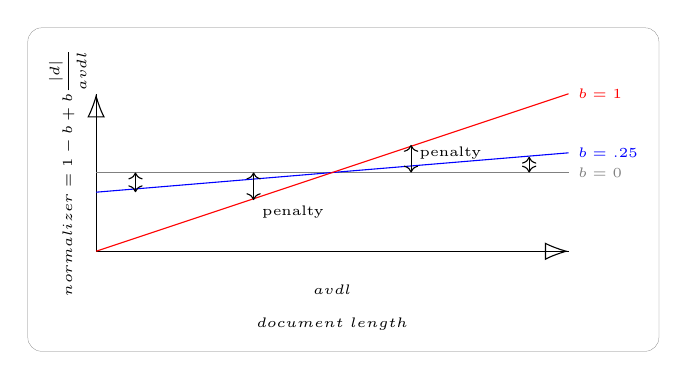
\begin{tikzpicture}
	[framed,background rectangle/.style={ultra thin, rounded corners=5pt, draw=gray}];

	%Axis
	\coordinate (x) at (6,0);
	\coordinate (y) at (0,2);
	\coordinate (o) at (0,0);
	\draw[-{Latex[length=3mm,open]}] (o)--(x); %node[right]{\large $document$ $length$};
	\draw (o) -- (x) node [midway, below, sloped, align=center, ] {\\ \tiny $avdl$ \\ \tiny $document$ $length$};
	\draw[-{Latex[length=3mm,open]}] (o)--(y);
	\draw (o) -- (y) node [midway, above, sloped, align=center] {\tiny $normalizer=1-b+b\dfrac{|d|}{avdl}$};

	\draw[gray] plot [domain=0:6] (\x,{1}) node[anchor=west]{\tiny $b = 0$} ;
	\draw[blue] plot [domain=0:6] (\x,{1-0.25+0.25*(\x/3)}) node[anchor=west]{\tiny $b = .25$} ;
	%\draw[red] plot [domain=0:6] (\x,{1-0.75+0.75*(\x/3)}) node[anchor=west]{\tiny $b = .75$} ;
	\draw[red] plot [domain=0:6] (\x,{1-1+1*(\x/3)}) node[anchor=west]{\tiny $b = 1$} ;

	\draw[<->] (4,1) -- (4,1.35);
	\node at (4.5,1.25) {\tiny penalty};
	\draw[<->] (5.5,1) -- (5.5,1.2);
	%\node at (5.7,1.25) {\tiny penalty};

	\draw[<->] (2,1) -- (2,0.65);
	\node at (2.5,0.50) {\tiny penalty};
	\draw[<->] (0.5,1) -- (0.5,0.75);
	%\node at (5.7,1.25) {\tiny penalty};
\end{tikzpicture}
\end{document}